% Nallino, Part II p. 236: the epicycle of the Moon with its centre A in the apogee of the excentric, redrawn from
% the print. The coordinates are those of a 400 dpi render of the figure (crop from x 112 pt, y 418 pt of the master
% page; y downward). E is the centre of the Earth, H and K the apogee and the perigee of the epicycle, G the Moon
% (HG = 60 degrees), M the foot of the perpendicular from G on EH; GM is dotted in the print.
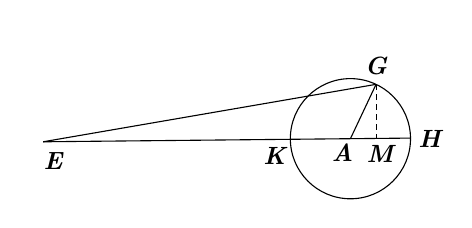
\begin{tikzpicture}[x=0.07mm,y=-0.07mm,line width=0.4pt,every node/.style={font=\bfseries\itshape\small,inner sep=1pt}]
\path (0,0);
\coordinate (E) at (28,207);
\coordinate (A) at (585.5,201.4);
\coordinate (H) at (694.5,200.3);
\coordinate (G) at (632,102.8);
\coordinate (M) at (632,200.9);
\draw (A) circle[radius=109];
\draw (E) -- (H);
\draw (E) -- (G);
\draw (A) -- (G);
\draw[dash pattern=on 2pt off 1.6pt] (G) -- (M);
\node at (632,69) {G};
\node at (729,202) {H};
\node at (571,227) {A};
\node at (639,229.5) {M};
\node at (448,232.5) {K};
\node at (46,241.5) {E};
\end{tikzpicture}
